% ------------------------------------------------------------------------
% -*-TeX-*- -*-Hard-*- Smart Wrapping
% ------------------------------------------------------------------------
\def\baselinestretch{1}

\chapter{Introduction}

\def\baselinestretch{1.44}

%%% ----------------------------------------------------------------------

This chapter introduces my dissertation topic: Comparing single-task learning (STL) and multi-task learning (MTL) models in predicting mental health symptoms in schizophrenia patients. It outlines the theoretical background, research motivations, and clearly defines the aim and objectives, forming the foundation for the technical analysis.

\smallskip

%%% ----------------------------------------------------------------------
\goodbreak
\section{Background}
Emil Kraepelin initially identified schizophrenia in the early 1900s. Emil labeled the condition as "dementia praecox," describing it as a gradually worsening mental illness with an unclear biological cause that typically starts during adolescence and results in significant and frequently permanent declines in cognitive and functional abilities ~ \citep{mcglashan1996early}~. Schizophrenia ranks among the 15 leading causes of disability globally ~\citep{james2020global}. Serious mental illnesses like schizophrenia, schizoaffective disorder, and severe bipolar disorder often involve psychosis, necessitating extended inpatient care and medical treatment. 

Psychosis disrupts clear thinking and reality perception due to delusional behavior, impacting a person's emotion, perception, behavior, and cognition \citep{wang2020predicting}. Schizophrenia affects fewer than 1\% of the general population, however, this figure rises to 10\% among people who have relatives who were diagnosed with the illness, such as parents or siblings. The majority of those with schizophrenia are not aggressive or violent but the risk of violence increases when the mental illness is not treated. In his study, \citet{Rasool2018SchizophreniaAO} revealed that genetic factors, environmental influences, and changes in brain structure are some of the leading factors causing Schizophrenia.

Developing nations are likely to experience slightly higher remission rates for schizophrenia, this may be due to simpler environmental conditions or stronger social support systems. The disorder often appears in early adulthood or late teens. People born in urban areas show a slightly higher prevalence of schizophrenia. For males, the peak onset age is between 15 and 25 years, while for females, it is delayed by about 3 to 5 years in females, leading to an equal prevalence among genders ~\citep{pearlson2000neurobiology}. However, a recent evaluation of data from 33 nations indicated that the prevalence of schizophrenia varies by geographic region ~\citep{Rasool2018SchizophreniaAO}. It impacts thinking, emotions, and behavior, often causing individuals to lose touch with reality and hear voices others do not. According to ~\citet{pearlson2000neurobiology}, in the United States, the yearly net medical expenses of schizophrenia have been projected to be \$37.7 \text{ billion}, with an indirect cost of \$117.3\text{billion}~ \citep{adler2020predicting}. This mental disorder is costly due to its early onset, chronic nature, and disabling effects, despite not being fatal. Symptoms fall into three categories: cognitive, negative, and positive, hallucinations and incoherent speech are examples of positive symptoms; decreased expressiveness and social disengagement are examples of negative symptoms. Worsening symptoms can lead to psychotic relapses, severely affecting personal relationships and employment. Early detection of relapse is crucial for timely intervention \citep{adler2020predicting}, whereas current clinical practices by clinicians are ineffective at early detection of behavioral precursors of schizophrenia. They are not scalable and fail to capture dynamic behavioral changes, resulting in interventions occurring at late stages of the disease like conventional face-to-face assessments \citep{canas2023counterfactual}. Brief Psychiatric Rating Scale (BPRS) used by clinicians to track symptoms of schizophrenia during routine clinical and conventional in-person evaluations usually take place every few months. However, between the visits, psychotic relapses might happen, significantly impacting the patient’s daily functioning and potentially endangering both the patient and their relatives. Developing tools to track symptom variations and detect early indicators of change is essential for assisting clinicians in making well-informed treatment decisions~ \citep{tseng2020using}. A computerized system that evaluates symptoms by modeling patient behavior might be valuable in predicting potential relapses, as shifts in behavior have been linked to the beginning of relapses~ \citep{zhou2022psychotic}. Smartphones and other mobile devices are being employed to gather data on users' behavior and physiological states to forecast mental health conditions \citep{tseng2020using}. At the same time, Machine learning (ML) has become a valuable tool, providing more objective and accurate detection methods \citep{thieme2020machine}. It has demonstrated numerous advantages in areas such as research, diagnosis, support, treatment, and clinical administration \citep{shatte2019machine}.  

One prominent example is the CrossCheck system, a sophisticated smartphone app developed for passive tracking and monitoring of symptoms related to schizophrenia \citep{adler2020predicting}. The CrossCheck study carried out at Zucker Hillside Hospital in New York City, monitored 150 outpatients diagnosed with schizophrenia over 12 months. The participants were assigned to two groups at random.: one group of 75 participants was assigned to use the CrossCheck smartphone, while the other 75 participants followed the usual treatment regimen. The study's objective was to forecast relapses, identified by clinical assessors, particularly focusing on the likelihood of a participant relapsing the following day.
The CrossCheck app utilized the Android activity API to determine if users were walking, stationary, cycling, tilting, or engaged in an unidentified activity. The app monitored conversation events (but not the content) and recorded daily sleep and wake times every 10 seconds during movement and 30 seconds when stationary. In addition, the GPS data was extracted and converted to track distinct locations and travel distances. The metadata on calls, texts, and phone unlocks were recorded and the ambient noise and light levels were also measured. The 10 Ecological Momentary Assessments (EMAs) questions were delivered via the Crosscheck app to the participants every Monday, Wednesday, and Friday to monitor schizophrenia symptoms. These symptoms included feelings of depression, stress, auditory hallucinations, visual hallucinations, fear of harm, calmness, sociability, sleep quality, mental clarity, and hopefulness. Responses were recorded on a scale from 0 (no symptom) to 3 (severe symptom) \citep{wang2016crosscheck}.  By integrating the passive sensing data with self-reported EMA,the researchers were able to predict the (EMAs) of participants. \citep{adler2020predicting} and \citep{wang2016crosscheck}. Previous studies utilizing the CrossCheck dataset revealed a significant relationship between variables such as sleep patterns, phone usage, mobility, conversations and self-reported schizophrenia symptoms. In his 2020 study, \citet{tseng2020using} demonstrated that the performance of multi-task learning (MTL) surpasses that of single-task learning STL when various algorithms are employed. This approach ensures that the model undergoes a balanced training process across both learning paradigms, allowing for a more robust comparison of their respective performances. Each symptom such as feelings of calmness, hope, sleeping, social, thinking and negative tasks such as feeling depressed, harm, seeing -things, hearing voices, and feeling stressed is trained independently in STL, whereas in MTL, several related tasks such as feeling calm, hopeful, sleeping, thinking are trained concurrently to improve generalization. For example, learning to predict feelings of calmness might also help improve the model's performance in predicting social engagement, as these tasks could share underlying psychological processes. This shared learning can result in better generalization of new, unseen data, leading to more reliable predictions in real-world scenarios. STL models, by focusing on isolated tasks, might overfit and fail to generalize well across different tasks. In complex mental health conditions like Schizophrenia, multi-task learning can capture the multifaceted nature of the disorder, potentially leading to more robust diagnostic tools and may offer a more comprehensive and accurate diagnostic solution offering insights that a series of independent STL models might overlook \citep{thieme2020machine}. 

This study builds on foundational research by advancing the analytical framework through the implementation of the Least Absolute Shrinkage and Selection Operator with Cross-Validation (LassoCV). LassoCV is adept at handling both Single Task Learning (STL) and Multi-Task Learning (MTL), through its MultiTaskLassoCV variant. The algorithm excels in feature selection and model regularization by shrinking less significant feature coefficients to zero, thereby enhancing model interpretability and robustness \citep{tseng2020using}. This research also investigates the impact of automatic alpha selection and hyperparameter tuning on the algorithm's performance. LassoCV autonomously selects the alpha parameter using cross-validation, optimizing the regularization strength without manual intervention. In contrast, hyperparameter tuning fine-tunes the alpha parameter through grid search or alternative optimization techniques to identify the optimal regularization strength.

In the context of high-dimensional datasets such as the Crosscheck dataset, it is hypothesized that the application of LassoCV and MultiTaskLassoCV will effectively address challenges such as multicollinearity, enhance model sparsity, and mitigate overfitting. These algorithms are anticipated to improve the model's generalization capabilities, thereby enhancing the reliability and interpretability of predictions. Moreover, it is posited that the consistent use of LassoCV and MultiTaskLassoCV will maximize data efficiency, streamline model tuning, and ensure methodological consistency, ultimately enhancing the comparability of results across diverse studies and datasets.
\section{Aim and Objectives}
\subsection{Aim}
To investigate the effectiveness of multi-task learning (MTL) using MultiTaskLassoCV compared to single-task learning (STL) using LassoCV in predicting Ecological Momentary Assessment (EMA) scores.
\subsection{Objectives}
The associated objectives are :
\begin{enumerate}
    \item To develop single-task learning models using LassoCV for EMA score prediction.
    \item To develop multi-task learning models using MultiTaskLassoCV for EMA score prediction.
    \item Compare the performance of the LassoCV and the MultiTaskLassoCV in terms of model prediction.
\end{enumerate}

\section{Research Project Work Plan}
The work plan used for this research project is as shown in Figure \ref{work}
\begin{figure}[H]
\centering
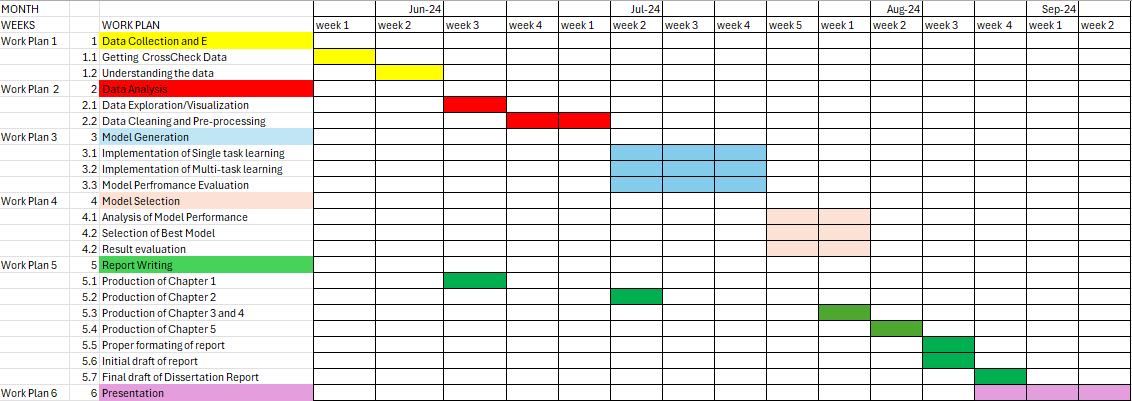
\includegraphics[scale=0.25]{work_plan.png}
\caption{Research Project Work Plan}
\label{work}
\end{figure}

\bigskip
\goodbreak


\section{Structure of Dissertation}
This dissertation is structured into five chapters, each progressively contributing to a comprehensive exploration of the research topic.

Chapter Breakdown
\begin{itemize}
\item Chapter 1: Introduction establishes the research context by outlining its background, motivation, and objectives.This outlines a clear framework for the dissertation.
\item Chapter 2:The Literature Review critically examines the existing body of research on machine learning applications across a range of mental health conditions, with a particular emphasis on its use in the prediction of Schizophrenia.Additionally, it explores the use of various both single-task and multi-task learning approaches, identifying knowledge gaps for further investigation.
\item Chapter 3: The Research Methodology section outlines the comprehensive approach taken to address the study’s objectives, which includes  data collection, pre-processing, and feature engineering. The section also covers both personalized and generalized modeling approaches, providing a thorough rationale for the chosen research design to ensure alignment with the study's goals.
\item Chapter 4: Results and Discussion presents the development and evaluation of generalized and personalized single-task and multitask learning models.Analyzes and discusses the performance comparison of these models.
\item Chapter 5: Conclusion summarizes key findings and assesses the achievement of research objectives. Discuss implications and provide recommendations for future research.
Each chapter is carefully structured to create a unified narrative that methodically tackles the research questions, providing a thorough and concentrated examination of the subject matter
\end{itemize}
\section{Summary}
The introduction chapter establishes the foundation for this research, which aims to compare the effectiveness of single-task learning (LassoCV) and multi-task learning (MultitaskLassoCV) models in predicting symptoms in Schizophrenia patients. Schizophrenia, a severe mental disorder, requires early and accurate detection to improve patient outcomes. This research is motivated by the need to develop more reliable diagnostic tools using multi-task learning which can lead to better and personalized treatment and overall patient well-being. Single-task learning, focusing on solving one specific task, and multi-task learning, which simultaneously addresses multiple related tasks, are the two approaches compared in this study. The hypothesis suggests that multi-task learning will provide superior diagnostic performance and generalization, especially given the complex nature of Schizophrenia. The dissertation is divided into five major chapters, each building on the previous chapters to give a comprehensive and in-depth exploration of the research topic. The subsequent chapters will cover a detailed literature review, methodology, results and discussion and conclusion.


%%% ----------------------------------------------------------------------
